% Textbook chapter section "8.2 Photosynthesis" (introductory biology). English, 3 pages.
% Features: learning objectives box, numbered subsections, labelled chloroplast diagram (tikz, captioned), the overall
% equation (mhchem, numbered), a light-response curve (pgfplots, captioned), key terms box, review questions at the end.
\documentclass[11pt,a4paper]{article}
\usepackage[T1]{fontenc}
\usepackage[utf8]{inputenc}
\usepackage{newtxtext,newtxmath}
\usepackage[scaled=0.9]{helvet}
\usepackage[english]{babel}
\usepackage[inner=2.8cm,outer=2.3cm,top=2.3cm,bottom=2.3cm]{geometry}
\usepackage{xcolor}
\usepackage{tikz}
\usetikzlibrary{calc}
\usepackage{pgfplots}
\pgfplotsset{compat=1.18}
\usepackage[version=4]{mhchem}
\usepackage{siunitx}
\usepackage{tcolorbox}
\usepackage{enumitem}
\usepackage{caption}
\usepackage{titlesec}
\usepackage{fancyhdr}
\usepackage{needspace}
\usepackage{microtype}

\definecolor{leaf}{HTML}{2E7D32}
\definecolor{leaflight}{HTML}{E8F3E8}
\setlength{\parindent}{1.2em}
\setlength{\parskip}{0.2em}
\captionsetup{font=small, labelfont={bf,sf}, labelsep=period, justification=raggedright, singlelinecheck=false}

% numbering "8.2", "8.2.1", "Figure 8.1", "(8.1)" as in chapter 8 of a textbook
\renewcommand{\thesection}{8.\arabic{section}}
\renewcommand{\thefigure}{8.\arabic{figure}}
\renewcommand{\theequation}{8.\arabic{equation}}
\setcounter{section}{1}
\titleformat{\section}{\sffamily\LARGE\bfseries\color{leaf}}{\thesection}{0.8em}{}
\titleformat{\subsection}{\sffamily\large\bfseries\color{leaf}}{\thesubsection}{0.6em}{}
\titlespacing*{\section}{0pt}{0.8em}{0.6em}
\titlespacing*{\subsection}{0pt}{1.1em}{0.3em}

\pagestyle{fancy}
\fancyhf{}
\renewcommand{\headrulewidth}{0.4pt}
\fancyhead[LE]{\sffamily\small\thepage \quad Chapter 8 \textperiodcentered{} Energy and Metabolism}
\fancyhead[RO]{\sffamily\small 8.2 Photosynthesis \quad\thepage}
\fancyfoot[C]{\sffamily\scriptsize Original teaching text for testing purposes.}

\begin{document}

\noindent{\sffamily\small\color{leaf}\textbf{CHAPTER 8 \quad ENERGY AND METABOLISM}}\\[-0.4em]
{\color{leaf}\rule{\linewidth}{0.8pt}}
\section{Photosynthesis: capturing light energy}

\begin{tcolorbox}[colback=leaflight, colframe=leaf, boxrule=0.6pt, arc=2pt, left=8pt, right=8pt, top=5pt, bottom=5pt,
  title={\sffamily\bfseries Learning objectives}, fonttitle=\sffamily, coltitle=white, colbacktitle=leaf]
After studying this section, you should be able to:
\begin{enumerate}[leftmargin=1.6em, itemsep=0.1em, label=\textbf{\arabic*.}]
  \item write the overall equation of photosynthesis and name its inputs and outputs;
  \item describe the structure of a chloroplast and locate the two stages of photosynthesis within it;
  \item explain why leaves look green and which wavelengths drive photosynthesis;
  \item read a light-response curve and explain the light compensation point and light saturation.
\end{enumerate}
\end{tcolorbox}

\subsection{The overall reaction}
Almost all life on Earth depends on photosynthesis, the process by which plants, algae and some bacteria use light
energy to build sugars from carbon dioxide and water. In plants, the process takes place in the leaf cells. A typical
mesophyll cell contains 30 to 70 chloroplasts. The overall reaction is summarised by Equation~8.1:
\begin{equation}
  \ce{6 CO2 + 6 H2O ->[\text{light}] C6H12O6 + 6 O2}
\end{equation}
Six molecules of carbon dioxide and six molecules of water are converted into one molecule of glucose and six molecules of
oxygen. The reaction stores energy: light energy ends up as chemical energy in the bonds of glucose. The oxygen
released comes from the water, not from the carbon dioxide.

\subsection{The chloroplast}
Photosynthesis takes place in chloroplasts, organelles that are about 4 to 6 micrometres long. Figure~8.1 shows their
structure. A chloroplast is surrounded by an \emph{outer membrane} and an \emph{inner membrane}. Inside is a fluid-filled
space, the \emph{stroma}, which contains enzymes, DNA and ribosomes. Embedded in the stroma is a third membrane system
made of flattened sacs called \emph{thylakoids}. Thylakoids are stacked like coins into \emph{grana} (singular:
granum). The thylakoid membranes carry the green pigment chlorophyll.

\begin{center}
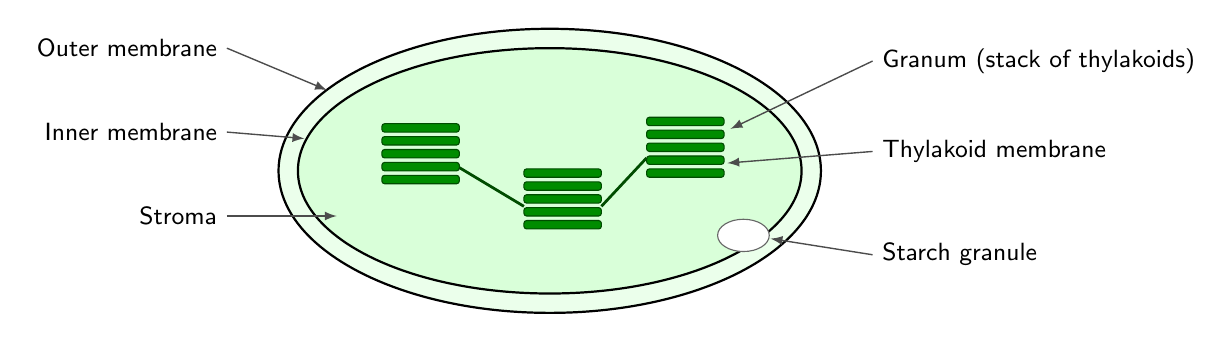
\begin{tikzpicture}[scale=0.82, font=\small, lab/.style={font=\small\sffamily}, lead/.style={-latex, black!70, line width=0.5pt}]
  % membranes
  \draw[thick, fill=green!8] (0,0) ellipse (4.2 and 2.2);
  \draw[thick, fill=green!15] (0,0) ellipse (3.9 and 1.9);
  % grana
  \foreach \x/\y in {-2.0/0.2, 0.2/-0.5, 2.1/0.3} {
    \foreach \i in {0,...,4} {
      \draw[fill=green!55!black, draw=green!30!black, rounded corners=1pt] (\x-0.6,\y+\i*0.2-0.4) rectangle (\x+0.6,\y+\i*0.2-0.27);
    }
  }
  % lamellae between grana
  \draw[green!30!black, line width=1pt] (-1.4,0.05) -- (-0.4,-0.55);
  \draw[green!30!black, line width=1pt] (0.8,-0.55) -- (1.5,0.2);
  % starch granule
  \draw[fill=white, draw=black!60] (3.0,-1.0) ellipse (0.4 and 0.25);
  % labels left
  \node[lab, anchor=east] at (-5.0,1.9) {Outer membrane};  \draw[lead] (-5.0,1.9) -- (-3.45,1.25);
  \node[lab, anchor=east] at (-5.0,0.6) {Inner membrane};  \draw[lead] (-5.0,0.6) -- (-3.8,0.5);
  \node[lab, anchor=east] at (-5.0,-0.7) {Stroma};         \draw[lead] (-5.0,-0.7) -- (-3.3,-0.7);
  % labels right
  \node[lab, anchor=west] at (5.0,1.7) {Granum (stack of thylakoids)};  \draw[lead] (5.0,1.7) -- (2.8,0.65);
  \node[lab, anchor=west] at (5.0,0.3) {Thylakoid membrane};            \draw[lead] (5.0,0.3) -- (2.75,0.12);
  \node[lab, anchor=west] at (5.0,-1.3) {Starch granule};               \draw[lead] (5.0,-1.3) -- (3.42,-1.05);
\end{tikzpicture}
\captionof{figure}{Structure of a chloroplast (schematic longitudinal section). The light-dependent reactions occur in the
thylakoid membranes; the Calvin cycle takes place in the stroma.}
\end{center}

\subsection{Light and pigments}
Sunlight is a mixture of wavelengths. Chlorophyll~\emph{a} absorbs light mainly in the blue-violet region (around
\qty{430}{nm}) and in the red region (around \qty{660}{nm}). It reflects green light, which is why leaves look green.
Accessory pigments such as carotenoids absorb other blue and green wavelengths and pass the energy on to chlorophyll.

\subsection{Stage 1: the light-dependent reactions}
The first stage of photosynthesis takes place in the thylakoid membranes. Light energy absorbed by chlorophyll
excites electrons, which are passed along a chain of electron carriers. To replace the lost electrons, water is
split (Equation~8.2), and oxygen is released as a by-product:
\begin{equation}
  \ce{2 H2O -> O2 + 4 H+ + 4 e-}
\end{equation}
As the electrons move along the chain, hydrogen ions are pumped into the interior of the thylakoids. The ions flow back
through the enzyme ATP synthase, which makes ATP. At the end of the chain, the electrons reduce the carrier \ce{NADP+}
to NADPH. The products of this stage are therefore \textbf{ATP}, \textbf{NADPH} and \textbf{oxygen}. No sugar is made yet.

\subsection{Stage 2: the Calvin cycle}
The second stage takes place in the stroma and does not need light directly. Using the ATP and NADPH from the first
stage, the Calvin cycle turns carbon dioxide into sugar. In the first step the enzyme \emph{rubisco} attaches
\ce{CO2} to a five-carbon sugar, ribulose bisphosphate (RuBP). The six-carbon product splits into two molecules of
3-phosphoglycerate, which are reduced to the three-carbon sugar G3P. Most G3P is used to regenerate RuBP; for every
three \ce{CO2} molecules fixed, one G3P leaves the cycle. To build one molecule of glucose the cycle must turn
six times and uses 18 molecules of ATP and 12 molecules of NADPH.

\subsection{Light intensity and the rate of photosynthesis}
How fast a leaf photosynthesises depends on the light it receives. Figure~8.2 shows the net uptake of carbon dioxide
by a sun plant and a shade plant at increasing light intensity. In the dark, both plants only respire, so the net
uptake is negative. As light intensity rises, photosynthesis increases until the carbon dioxide taken up for
photosynthesis exactly equals the carbon dioxide released by respiration. This point is the \emph{light compensation
point}: about 40 $\mu$mol photons m$^{-2}$ s$^{-1}$ for the sun plant and about 15 for the shade plant. At higher
intensities the curve rises almost linearly at first and then levels off. The sun plant reaches \emph{light
saturation} at about 1000 and a maximum net uptake of about 18 $\mu$mol CO$_2$ m$^{-2}$ s$^{-1}$; the shade plant is
saturated at about 400 with a maximum of about 8. Above saturation, another factor limits the rate, such as the
supply of \ce{CO2} or the amount of rubisco.

\begin{center}
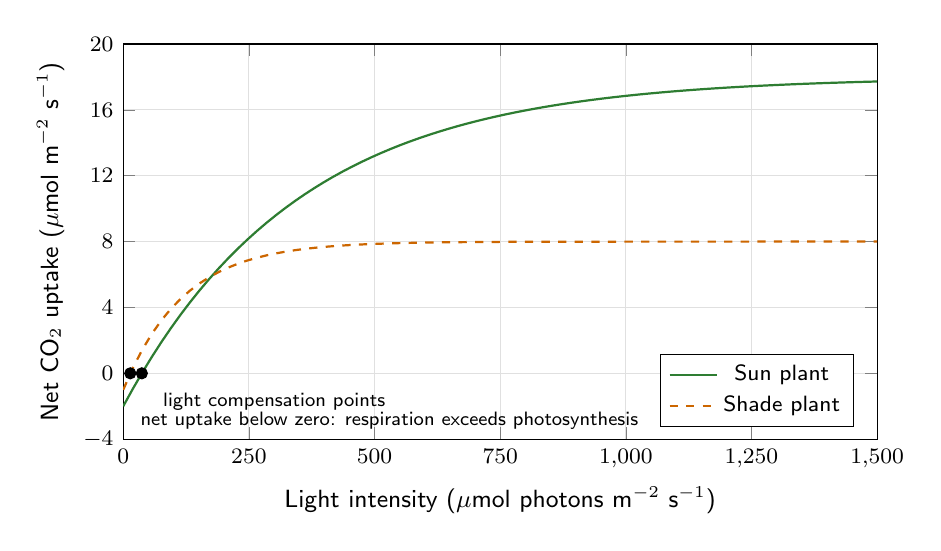
\begin{tikzpicture}
\begin{axis}[
    width=0.92\linewidth, height=6.6cm,
    xlabel={Light intensity ($\mu$mol photons m$^{-2}$ s$^{-1}$)},
    ylabel={Net CO$_2$ uptake ($\mu$mol m$^{-2}$ s$^{-1}$)},
    xmin=0, xmax=1500, ymin=-4, ymax=20,
    xtick={0,250,500,750,1000,1250,1500}, ytick={-4,0,4,8,12,16,20},
    grid=both, grid style={black!12}, tick label style={font=\sffamily\footnotesize}, label style={font=\sffamily\small},
    legend pos=south east, legend style={font=\sffamily\footnotesize}]
  \addplot[domain=0:1500, samples=80, thick, leaf] {20*(1-exp(-x/350)) - 2};
  \addlegendentry{Sun plant}
  \addplot[domain=0:1500, samples=80, thick, orange!80!black, dashed] {9*(1-exp(-x/120)) - 1};
  \addlegendentry{Shade plant}
  \addplot[only marks, mark=*, mark size=2pt, black] coordinates {(37,0) (14,0)};
  \node[font=\sffamily\scriptsize, anchor=north west] at (axis cs:60,-0.6) {light compensation points};
  \node[font=\sffamily\scriptsize, anchor=west] at (axis cs:15,-2.9) {net uptake below zero: respiration exceeds photosynthesis};
\end{axis}
\end{tikzpicture}
\captionof{figure}{Light-response curves of a sun plant (solid) and a shade plant (dashed). The dots mark the light
compensation points, where net carbon dioxide uptake is zero.}
\end{center}

% ---- Key terms -------------------------------------------------------------------------------------
\Needspace{14\baselineskip}
\begin{tcolorbox}[colback=leaflight, colframe=leaf, boxrule=0.6pt, arc=2pt, left=8pt, right=8pt, top=5pt, bottom=5pt,
  title={\sffamily\bfseries Key terms}, fonttitle=\sffamily, coltitle=white, colbacktitle=leaf]
\small
\begin{description}[leftmargin=0pt, labelindent=0pt, itemsep=0.15em, parsep=0pt, font=\bfseries]
  \item[photosynthesis] process that converts light energy, carbon dioxide and water into glucose and oxygen
  \item[chlorophyll] green pigment in the thylakoid membranes that absorbs red and blue light
  \item[stroma] fluid-filled space inside the chloroplast where the Calvin cycle takes place
  \item[thylakoid, granum] flattened membrane sac; a stack of thylakoids
  \item[ATP, NADPH] energy-rich molecules made in stage 1 and used in stage 2
  \item[Calvin cycle] series of reactions that fixes carbon dioxide into sugar, using ATP and NADPH
  \item[rubisco] enzyme that attaches carbon dioxide to RuBP
  \item[light compensation point] light intensity at which net carbon dioxide uptake is zero
\end{description}
\end{tcolorbox}

% ---- Review questions ------------------------------------------------------------------------------
\subsection*{\sffamily\large\bfseries\color{leaf} Review questions}
\begin{enumerate}[leftmargin=1.8em, itemsep=0.3em, label=\textbf{Q\arabic*}]
  \item State the overall equation of photosynthesis in words. Where does the oxygen released come from?
  \item In which part of the chloroplast do the light-dependent reactions take place, and what are their three products?
  \item Why do leaves look green, and which wavelengths does chlorophyll absorb best?
  \item Use Figure~8.2 to explain what happens at the light compensation point. Which plant has the lower one?
  \item A student claims that the Calvin cycle does not need light. Explain in what sense she is right and in what sense
        she is wrong.
  \item How many molecules of ATP and NADPH are needed to make one molecule of glucose, and why?
\end{enumerate}

\end{document}
